%%%%%%%%%%%%%%%%%%%%%%%%%%%%%%%%%%%%%%%%%%%%%%%%%%%%%%%%%%%%%%%%%%%%%%%%%%%%%%%%%%%%%%%%%%%%%%%%%%%%%%%%%%%%%%%%%%%%%%%%%%%%%%%%%%%%%%%%%%%%%%%%%%%%%%%%%%%%%%%%%%%
% Written By Michael Brodskiy
% Class: Circuits & Signals: Biomedical Applications
% Professor: N. Sun
%%%%%%%%%%%%%%%%%%%%%%%%%%%%%%%%%%%%%%%%%%%%%%%%%%%%%%%%%%%%%%%%%%%%%%%%%%%%%%%%%%%%%%%%%%%%%%%%%%%%%%%%%%%%%%%%%%%%%%%%%%%%%%%%%%%%%%%%%%%%%%%%%%%%%%%%%%%%%%%%%%%

\include{Includes.tex}

\title{Thevnin and Norton Equivalents}
\date{\today}
\author{Michael Brodskiy\\ \small Professor: N. Sun}

\begin{document}

\maketitle

\begin{itemize}

  \item Circuit Equivalence

    \begin{itemize}

      \item If there are two circuits, and the same voltage, $v_a$ is applied to both, if $I_A=I_B$ then the circuits are considered equivalent

      \item Same thing for same current applied and same voltage output

    \end{itemize}

  \item Resistor Equivalence

    \begin{itemize}

      \item Resistors can be connected in circuits like a delta connection

      \item As well as a Y connection

      \item A delta connection can be transformed into a Y connection and vice versa using transformation technique

      \item This will often help in circuits

    \end{itemize}

    \begin{figure}[H]
      \centering
      \tikzset{every picture/.style={line width=0.75pt}} %set default line width to 0.75pt        

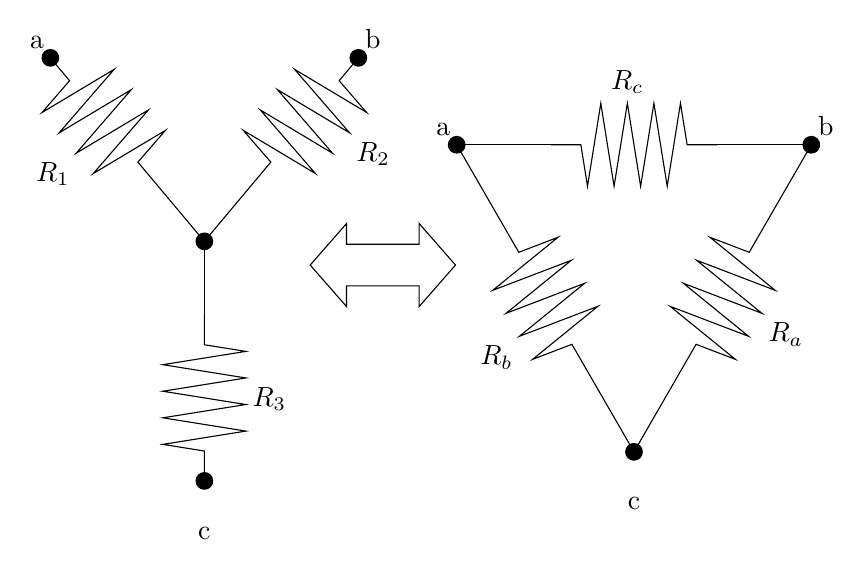
\begin{tikzpicture}[x=0.75pt,y=0.75pt,yscale=-1,xscale=1]
%uncomment if require: \path (0,420); %set diagram left start at 0, and has height of 420

%Shape: Resistor [id:dp8649111880326505] 
\draw   (219,197) -- (219,211.4) -- (239,214.6) -- (199,221) -- (239,227.4) -- (199,233.8) -- (239,240.2) -- (199,246.6) -- (239,253) -- (199,259.4) -- (219,262.6) -- (219,277) ;
%Shape: Resistor [id:dp9942934984762448] 
\draw   (241.77,134.44) -- (251.02,123.41) -- (237.76,108.11) -- (272.52,128.91) -- (245.99,98.3) -- (280.74,119.11) -- (254.22,88.5) -- (288.97,109.3) -- (262.44,78.69) -- (297.2,99.5) -- (283.94,84.19) -- (293.19,73.16) ;
%Shape: Resistor [id:dp85596491014942] 
\draw   (144.81,73.16) -- (154.06,84.19) -- (140.8,99.5) -- (175.56,78.69) -- (149.03,109.3) -- (183.78,88.5) -- (157.26,119.11) -- (192.01,98.3) -- (165.48,128.91) -- (200.24,108.11) -- (186.98,123.41) -- (196.23,134.44) ;
%Straight Lines [id:da23101519075185095] 
\draw    (219,161.58) -- (219,197) ;
%Straight Lines [id:da3890276784519242] 
\draw    (219,161.58) -- (196.23,134.44) ;
%Straight Lines [id:da7445936080781037] 
\draw    (219,161.58) -- (241.77,134.44) ;
%Shape: Circle [id:dp8383610920721991] 
\draw  [fill={rgb, 255:red, 0; green, 0; blue, 0 }  ,fill opacity=1 ] (215,161.58) .. controls (215,159.37) and (216.79,157.58) .. (219,157.58) .. controls (221.21,157.58) and (223,159.37) .. (223,161.58) .. controls (223,163.79) and (221.21,165.58) .. (219,165.58) .. controls (216.79,165.58) and (215,163.79) .. (215,161.58) -- cycle ;
%Shape: Circle [id:dp09797149394585802] 
\draw  [fill={rgb, 255:red, 0; green, 0; blue, 0 }  ,fill opacity=1 ] (289.19,73.16) .. controls (289.19,70.95) and (290.98,69.16) .. (293.19,69.16) .. controls (295.4,69.16) and (297.19,70.95) .. (297.19,73.16) .. controls (297.19,75.37) and (295.4,77.16) .. (293.19,77.16) .. controls (290.98,77.16) and (289.19,75.37) .. (289.19,73.16) -- cycle ;
%Shape: Circle [id:dp7483012020928743] 
\draw  [fill={rgb, 255:red, 0; green, 0; blue, 0 }  ,fill opacity=1 ] (140.81,73.16) .. controls (140.81,70.95) and (142.6,69.16) .. (144.81,69.16) .. controls (147.02,69.16) and (148.81,70.95) .. (148.81,73.16) .. controls (148.81,75.37) and (147.02,77.16) .. (144.81,77.16) .. controls (142.6,77.16) and (140.81,75.37) .. (140.81,73.16) -- cycle ;
%Shape: Circle [id:dp03389973177254291] 
\draw  [fill={rgb, 255:red, 0; green, 0; blue, 0 }  ,fill opacity=1 ] (215,277) .. controls (215,274.79) and (216.79,273) .. (219,273) .. controls (221.21,273) and (223,274.79) .. (223,277) .. controls (223,279.21) and (221.21,281) .. (219,281) .. controls (216.79,281) and (215,279.21) .. (215,277) -- cycle ;
%Shape: Resistor [id:dp7459678467673858] 
\draw   (386,115.05) -- (400.4,115.05) -- (403.6,135.05) -- (410,95.05) -- (416.4,135.05) -- (422.8,95.05) -- (429.2,135.05) -- (435.6,95.05) -- (442,135.05) -- (448.4,95.05) -- (451.6,115.05) -- (466,115.05) ;
%Shape: Resistor [id:dp8943386559820388] 
\draw   (448.71,223.66) -- (455.91,211.19) -- (474.83,218.42) -- (443.39,192.88) -- (481.23,207.34) -- (449.79,181.79) -- (487.63,196.25) -- (456.19,170.71) -- (494.03,185.17) -- (462.59,159.62) -- (481.51,166.85) -- (488.71,154.38) ;
%Straight Lines [id:da980522130958174] 
\draw    (386,115.05) -- (340.58,115.05) ;
%Straight Lines [id:da25013706782614387] 
\draw    (511.42,115.05) -- (466,115.05) ;
%Straight Lines [id:da024405235938776526] 
\draw    (511.42,115.05) -- (488.71,154.38) ;
%Straight Lines [id:da41196160100547097] 
\draw    (448.71,223.66) -- (426,263) ;
%Shape: Resistor [id:dp8933369509641274] 
\draw   (363.29,154.38) -- (370.49,166.85) -- (389.41,159.62) -- (357.97,185.17) -- (395.81,170.71) -- (364.37,196.25) -- (402.21,181.79) -- (370.77,207.34) -- (408.61,192.88) -- (377.17,218.42) -- (396.09,211.19) -- (403.29,223.66) ;
%Straight Lines [id:da14103113154035296] 
\draw    (426,263) -- (403.29,223.66) ;
%Straight Lines [id:da012997480095768843] 
\draw    (363.29,154.38) -- (340.58,115.05) ;
%Shape: Circle [id:dp5583976916907458] 
\draw  [fill={rgb, 255:red, 0; green, 0; blue, 0 }  ,fill opacity=1 ] (336.58,115.05) .. controls (336.58,117.26) and (338.37,119.05) .. (340.58,119.05) .. controls (342.79,119.05) and (344.58,117.26) .. (344.58,115.05) .. controls (344.58,112.84) and (342.79,111.05) .. (340.58,111.05) .. controls (338.37,111.05) and (336.58,112.84) .. (336.58,115.05) -- cycle ;
%Shape: Circle [id:dp044013820240165646] 
\draw  [fill={rgb, 255:red, 0; green, 0; blue, 0 }  ,fill opacity=1 ] (422,263) .. controls (422,265.21) and (423.79,267) .. (426,267) .. controls (428.21,267) and (430,265.21) .. (430,263) .. controls (430,260.79) and (428.21,259) .. (426,259) .. controls (423.79,259) and (422,260.79) .. (422,263) -- cycle ;
%Shape: Circle [id:dp9756959473863265] 
\draw  [fill={rgb, 255:red, 0; green, 0; blue, 0 }  ,fill opacity=1 ] (507.42,115.05) .. controls (507.42,117.26) and (509.21,119.05) .. (511.42,119.05) .. controls (513.63,119.05) and (515.42,117.26) .. (515.42,115.05) .. controls (515.42,112.84) and (513.63,111.05) .. (511.42,111.05) .. controls (509.21,111.05) and (507.42,112.84) .. (507.42,115.05) -- cycle ;
%Left Right Arrow [id:dp6518423274771699] 
\draw   (270,173) -- (287.5,153) -- (287.5,163) -- (322.5,163) -- (322.5,153) -- (340,173) -- (322.5,193) -- (322.5,183) -- (287.5,183) -- (287.5,193) -- cycle ;

% Text Node
\draw (142.81,70.16) node [anchor=south east] [inner sep=0.75pt]   [align=left] {a};
% Text Node
\draw (295.19,70.16) node [anchor=south west] [inner sep=0.75pt]   [align=left] {b};
% Text Node
\draw (219,298) node [anchor=north] [inner sep=0.75pt]   [align=left] {c};
% Text Node
\draw (489.63,199.65) node [anchor=north west][inner sep=0.75pt]    {$R_{a}$};
% Text Node
\draw (368.77,210.74) node [anchor=north east] [inner sep=0.75pt]    {$R_{b}$};
% Text Node
\draw (422.8,91.65) node [anchor=south] [inner sep=0.75pt]    {$R_{c}$};
% Text Node
\draw (338.58,112.05) node [anchor=south east] [inner sep=0.75pt]   [align=left] {a};
% Text Node
\draw (513.42,112.05) node [anchor=south west] [inner sep=0.75pt]   [align=left] {b};
% Text Node
\draw (426,284) node [anchor=north] [inner sep=0.75pt]   [align=left] {c};
% Text Node
\draw (155.26,122.51) node [anchor=north east] [inner sep=0.75pt]    {$R_{1}$};
% Text Node
\draw (290.97,112.7) node [anchor=north west][inner sep=0.75pt]    {$R_{2}$};
% Text Node
\draw (241,230.8) node [anchor=north west][inner sep=0.75pt]    {$R_{3}$};


\end{tikzpicture}

      \caption{Delta and Y Circuit Configurations}
      \label{fig:1}
    \end{figure}

  \item Transformations can be established from one to the other, as shown in Figure 1, using the following

    $$\boxed{R_1=\frac{R_bR_c}{R_a+R_b+R_c},\,\,\,\,\,\,\,\,R_2=\frac{R_cR_a}{R_a+R_b+R_c},\,\,\,\,\,\,\,\,R_3=\frac{R_aR_b}{R_a+R_b+R_c}}$$
    $$\boxed{R_a=\frac{R_1R_2+R_2R_3+R_3R_1}{R_1},\,\,\,\,\,\,\,\,R_2=\frac{R_1R_2+R_2R_3+R_3R_1}{R_2},\,\,\,\,\,\,\,\,R_c=\frac{R_1R_2+R_2R_3+R_3R_1}{R_3}}$$

  \item A voltage source with a series resistor can be transformed into a current source with a resistor in parallel, as shown in Figure 2

    \begin{figure}[H]
      \centering
      \tikzset{every picture/.style={line width=0.75pt}} %set default line width to 0.75pt        

\begin{tikzpicture}[x=0.75pt,y=0.75pt,yscale=-1,xscale=1]
%uncomment if require: \path (0,508); %set diagram left start at 0, and has height of 508

%Shape: Output [id:dp4761018043956171] 
\draw   (119,130) .. controls (135.57,130) and (149,142.98) .. (149,159) .. controls (149,175.02) and (135.57,188) .. (119,188) .. controls (102.43,188) and (89,175.02) .. (89,159) .. controls (89,142.98) and (102.43,130) .. (119,130) -- cycle (119,101) -- (119,130) (119,217) -- (119,188) ;
%Straight Lines [id:da18038673316668685] 
\draw    (260.42,217) -- (119,217) ;
%Shape: Resistor [id:dp49094225036149086] 
\draw   (119,101) -- (144.46,101) -- (150.11,81) -- (161.43,121) -- (172.74,81) -- (184.05,121) -- (195.37,81) -- (206.68,121) -- (217.99,81) -- (229.31,121) -- (234.97,101) -- (260.42,101) ;
%Shape: Circle [id:dp7252316282946523] 
\draw  [fill={rgb, 255:red, 0; green, 0; blue, 0 }  ,fill opacity=1 ] (256.92,101) .. controls (256.92,99.07) and (258.49,97.5) .. (260.42,97.5) .. controls (262.35,97.5) and (263.92,99.07) .. (263.92,101) .. controls (263.92,102.93) and (262.35,104.5) .. (260.42,104.5) .. controls (258.49,104.5) and (256.92,102.93) .. (256.92,101) -- cycle ;
%Shape: Circle [id:dp7082112398028335] 
\draw  [fill={rgb, 255:red, 0; green, 0; blue, 0 }  ,fill opacity=1 ] (256.92,217) .. controls (256.92,215.07) and (258.49,213.5) .. (260.42,213.5) .. controls (262.35,213.5) and (263.92,215.07) .. (263.92,217) .. controls (263.92,218.93) and (262.35,220.5) .. (260.42,220.5) .. controls (258.49,220.5) and (256.92,218.93) .. (256.92,217) -- cycle ;
%Shape: Output [id:dp31169582279695573] 
\draw   (119,349) .. controls (135.57,349) and (149,361.98) .. (149,378) .. controls (149,394.02) and (135.57,407) .. (119,407) .. controls (102.43,407) and (89,394.02) .. (89,378) .. controls (89,361.98) and (102.43,349) .. (119,349) -- cycle (119,320) -- (119,349) (119,436) -- (119,407) ;
%Straight Lines [id:da40535921970588173] 
\draw    (260.42,436) -- (119,436) ;
%Shape: Resistor [id:dp4721611778600978] 
\draw   (260.42,320) -- (260.42,340.88) -- (280.42,345.52) -- (240.42,354.8) -- (280.42,364.08) -- (240.42,373.36) -- (280.42,382.64) -- (240.42,391.92) -- (280.42,401.2) -- (240.42,410.48) -- (260.42,415.12) -- (260.42,436) ;
%Straight Lines [id:da9415238641357673] 
\draw    (401.84,320) -- (260.42,320) ;
%Straight Lines [id:da3487179058682581] 
\draw    (401.84,436) -- (260.42,436) ;
%Shape: Circle [id:dp7676950007550718] 
\draw  [fill={rgb, 255:red, 0; green, 0; blue, 0 }  ,fill opacity=1 ] (256.92,320) .. controls (256.92,318.07) and (258.49,316.5) .. (260.42,316.5) .. controls (262.35,316.5) and (263.92,318.07) .. (263.92,320) .. controls (263.92,321.93) and (262.35,323.5) .. (260.42,323.5) .. controls (258.49,323.5) and (256.92,321.93) .. (256.92,320) -- cycle ;
%Shape: Circle [id:dp7754991479549254] 
\draw  [fill={rgb, 255:red, 0; green, 0; blue, 0 }  ,fill opacity=1 ] (256.92,436) .. controls (256.92,434.07) and (258.49,432.5) .. (260.42,432.5) .. controls (262.35,432.5) and (263.92,434.07) .. (263.92,436) .. controls (263.92,437.93) and (262.35,439.5) .. (260.42,439.5) .. controls (258.49,439.5) and (256.92,437.93) .. (256.92,436) -- cycle ;
%Straight Lines [id:da8126562773083341] 
\draw    (260.42,320) -- (119,320) ;
%Shape: Circle [id:dp749150677492284] 
\draw  [fill={rgb, 255:red, 0; green, 0; blue, 0 }  ,fill opacity=1 ] (398.34,320) .. controls (398.34,318.07) and (399.91,316.5) .. (401.84,316.5) .. controls (403.78,316.5) and (405.34,318.07) .. (405.34,320) .. controls (405.34,321.93) and (403.78,323.5) .. (401.84,323.5) .. controls (399.91,323.5) and (398.34,321.93) .. (398.34,320) -- cycle ;
%Shape: Circle [id:dp8460624756938435] 
\draw  [fill={rgb, 255:red, 0; green, 0; blue, 0 }  ,fill opacity=1 ] (398.34,436) .. controls (398.34,434.07) and (399.91,432.5) .. (401.84,432.5) .. controls (403.78,432.5) and (405.34,434.07) .. (405.34,436) .. controls (405.34,437.93) and (403.78,439.5) .. (401.84,439.5) .. controls (399.91,439.5) and (398.34,437.93) .. (398.34,436) -- cycle ;
%Straight Lines [id:da6858366079722793] 
\draw [line width=1.5]    (119,393) -- (119,362) ;
\draw [shift={(119,359)}, rotate = 90] [color={rgb, 255:red, 0; green, 0; blue, 0 }  ][line width=1.5]    (14.21,-4.28) .. controls (9.04,-1.82) and (4.3,-0.39) .. (0,0) .. controls (4.3,0.39) and (9.04,1.82) .. (14.21,4.28)   ;
%Up Down Arrow [id:dp13938108550459183] 
\draw   (186,251.5) -- (210,234) -- (234,251.5) -- (222,251.5) -- (222,286.5) -- (234,286.5) -- (210,304) -- (186,286.5) -- (198,286.5) -- (198,251.5) -- cycle ;

% Text Node
\draw (87,159) node [anchor=east] [inner sep=0.75pt]   [align=left] {$\displaystyle v_{s}$};
% Text Node
\draw (193.37,78) node [anchor=south east] [inner sep=0.75pt]   [align=left] {$\displaystyle R$};
% Text Node
\draw (119,133) node [anchor=north] [inner sep=0.75pt]   [align=left] {\begin{minipage}[lt]{8.68pt}\setlength\topsep{0pt}
\begin{center}
+
\end{center}

\end{minipage}};
% Text Node
\draw (119,185) node [anchor=south] [inner sep=0.75pt]   [align=left] {$\displaystyle -$};
% Text Node
\draw (87,378) node [anchor=east] [inner sep=0.75pt]   [align=left] {$\displaystyle i_{s}$};
% Text Node
\draw (282.42,367.08) node [anchor=north west][inner sep=0.75pt]   [align=left] {$\displaystyle R$};
% Text Node
\draw (265.92,104) node [anchor=north west][inner sep=0.75pt]   [align=left] {a};
% Text Node
\draw (407.34,323) node [anchor=north west][inner sep=0.75pt]   [align=left] {a};
% Text Node
\draw (265.92,220) node [anchor=north west][inner sep=0.75pt]   [align=left] {b};
% Text Node
\draw (407.34,439) node [anchor=north west][inner sep=0.75pt]   [align=left] {b};


\end{tikzpicture}

      \caption{Converting Between Voltage and Current}
      \label{fig:2}
    \end{figure}

  \item A parallel resistor with a voltage source can be removed (replaced by an open) for transformation, as shown in Figure 3

    \begin{figure}[H]
      \centering
      \tikzset{every picture/.style={line width=0.75pt}} %set default line width to 0.75pt        

\begin{tikzpicture}[x=0.75pt,y=0.75pt,yscale=-1,xscale=1]
%uncomment if require: \path (0,642); %set diagram left start at 0, and has height of 642

%Shape: Output [id:dp4761018043956171] 
\draw   (254,86) .. controls (270.57,86) and (284,98.98) .. (284,115) .. controls (284,131.02) and (270.57,144) .. (254,144) .. controls (237.43,144) and (224,131.02) .. (224,115) .. controls (224,98.98) and (237.43,86) .. (254,86) -- cycle (254,57) -- (254,86) (254,173) -- (254,144) ;
%Straight Lines [id:da18038673316668685] 
\draw    (395.42,173) -- (254,173) ;
%Shape: Resistor [id:dp49094225036149086] 
\draw   (395.42,57) -- (420.88,57) -- (426.53,37) -- (437.85,77) -- (449.16,37) -- (460.48,77) -- (471.79,37) -- (483.1,77) -- (494.42,37) -- (505.73,77) -- (511.39,57) -- (536.84,57) ;
%Shape: Circle [id:dp7252316282946523] 
\draw  [fill={rgb, 255:red, 0; green, 0; blue, 0 }  ,fill opacity=1 ] (391.92,57) .. controls (391.92,55.07) and (393.49,53.5) .. (395.42,53.5) .. controls (397.35,53.5) and (398.92,55.07) .. (398.92,57) .. controls (398.92,58.93) and (397.35,60.5) .. (395.42,60.5) .. controls (393.49,60.5) and (391.92,58.93) .. (391.92,57) -- cycle ;
%Shape: Circle [id:dp7082112398028335] 
\draw  [fill={rgb, 255:red, 0; green, 0; blue, 0 }  ,fill opacity=1 ] (391.92,173) .. controls (391.92,171.07) and (393.49,169.5) .. (395.42,169.5) .. controls (397.35,169.5) and (398.92,171.07) .. (398.92,173) .. controls (398.92,174.93) and (397.35,176.5) .. (395.42,176.5) .. controls (393.49,176.5) and (391.92,174.93) .. (391.92,173) -- cycle ;
%Shape: Output [id:dp6368500887380681] 
\draw   (256,356) .. controls (272.57,356) and (286,368.98) .. (286,385) .. controls (286,401.02) and (272.57,414) .. (256,414) .. controls (239.43,414) and (226,401.02) .. (226,385) .. controls (226,368.98) and (239.43,356) .. (256,356) -- cycle (256,327) -- (256,356) (256,443) -- (256,414) ;
%Straight Lines [id:da25378864334436835] 
\draw    (397.42,443) -- (256,443) ;
%Shape: Resistor [id:dp10671543731782762] 
\draw   (256,327) -- (281.46,327) -- (287.11,307) -- (298.43,347) -- (309.74,307) -- (321.05,347) -- (332.37,307) -- (343.68,347) -- (354.99,307) -- (366.31,347) -- (371.97,327) -- (397.42,327) ;
%Shape: Circle [id:dp522496327022093] 
\draw  [fill={rgb, 255:red, 0; green, 0; blue, 0 }  ,fill opacity=1 ] (393.92,327) .. controls (393.92,325.07) and (395.49,323.5) .. (397.42,323.5) .. controls (399.35,323.5) and (400.92,325.07) .. (400.92,327) .. controls (400.92,328.93) and (399.35,330.5) .. (397.42,330.5) .. controls (395.49,330.5) and (393.92,328.93) .. (393.92,327) -- cycle ;
%Shape: Circle [id:dp8014445694731585] 
\draw  [fill={rgb, 255:red, 0; green, 0; blue, 0 }  ,fill opacity=1 ] (393.92,443) .. controls (393.92,441.07) and (395.49,439.5) .. (397.42,439.5) .. controls (399.35,439.5) and (400.92,441.07) .. (400.92,443) .. controls (400.92,444.93) and (399.35,446.5) .. (397.42,446.5) .. controls (395.49,446.5) and (393.92,444.93) .. (393.92,443) -- cycle ;
%Straight Lines [id:da18260678273306796] 
\draw    (395.42,57) -- (254,57) ;
%Shape: Resistor [id:dp684354118396199] 
\draw   (395.42,57) -- (395.42,77.88) -- (415.42,82.52) -- (375.42,91.8) -- (415.42,101.08) -- (375.42,110.36) -- (415.42,119.64) -- (375.42,128.92) -- (415.42,138.2) -- (375.42,147.48) -- (395.42,152.12) -- (395.42,173) ;
%Straight Lines [id:da8845127840871825] 
\draw    (536.84,173) -- (395.42,173) ;
%Shape: Circle [id:dp9978288916988585] 
\draw  [fill={rgb, 255:red, 0; green, 0; blue, 0 }  ,fill opacity=1 ] (533.34,57) .. controls (533.34,55.07) and (534.91,53.5) .. (536.84,53.5) .. controls (538.78,53.5) and (540.34,55.07) .. (540.34,57) .. controls (540.34,58.93) and (538.78,60.5) .. (536.84,60.5) .. controls (534.91,60.5) and (533.34,58.93) .. (533.34,57) -- cycle ;
%Shape: Circle [id:dp9681776211546007] 
\draw  [fill={rgb, 255:red, 0; green, 0; blue, 0 }  ,fill opacity=1 ] (533.34,173) .. controls (533.34,171.07) and (534.91,169.5) .. (536.84,169.5) .. controls (538.78,169.5) and (540.34,171.07) .. (540.34,173) .. controls (540.34,174.93) and (538.78,176.5) .. (536.84,176.5) .. controls (534.91,176.5) and (533.34,174.93) .. (533.34,173) -- cycle ;
%Up Down Arrow [id:dp03182684902749244] 
\draw   (320,209.5) -- (340.5,193) -- (361,209.5) -- (350.75,209.5) -- (350.75,242.5) -- (361,242.5) -- (340.5,259) -- (320,242.5) -- (330.25,242.5) -- (330.25,209.5) -- cycle ;

% Text Node
\draw (222,115) node [anchor=east] [inner sep=0.75pt]   [align=left] {$\displaystyle v_{s}$};
% Text Node
\draw (469.79,34) node [anchor=south east] [inner sep=0.75pt]   [align=left] {$\displaystyle R$};
% Text Node
\draw (254,89) node [anchor=north] [inner sep=0.75pt]   [align=left] {\begin{minipage}[lt]{8.68pt}\setlength\topsep{0pt}
\begin{center}
+
\end{center}

\end{minipage}};
% Text Node
\draw (254,141) node [anchor=south] [inner sep=0.75pt]   [align=left] {$\displaystyle -$};
% Text Node
\draw (224,385) node [anchor=east] [inner sep=0.75pt]   [align=left] {$\displaystyle v_{s}$};
% Text Node
\draw (330.37,304) node [anchor=south east] [inner sep=0.75pt]   [align=left] {$\displaystyle R$};
% Text Node
\draw (256,359) node [anchor=north] [inner sep=0.75pt]   [align=left] {\begin{minipage}[lt]{8.68pt}\setlength\topsep{0pt}
\begin{center}
+
\end{center}

\end{minipage}};
% Text Node
\draw (256,411) node [anchor=south] [inner sep=0.75pt]   [align=left] {$\displaystyle -$};
% Text Node
\draw (402.92,330) node [anchor=north west][inner sep=0.75pt]   [align=left] {a};
% Text Node
\draw (402.92,446) node [anchor=north west][inner sep=0.75pt]   [align=left] {b};


\end{tikzpicture}

      \caption{Converting Voltage Sources}
      \label{fig:3}
    \end{figure}

  \item A series resistor with a current source can be removed (replaced by a short) for transformation, as shown in Figure 4

    \begin{figure}[H]
      \centering
      \tikzset{every picture/.style={line width=0.75pt}} %set default line width to 0.75pt        

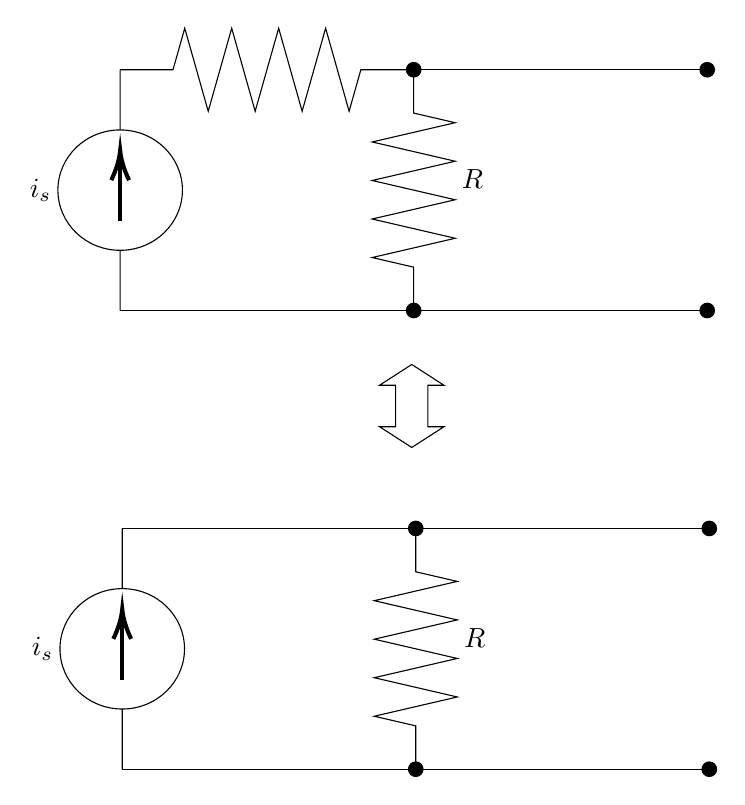
\begin{tikzpicture}[x=0.75pt,y=0.75pt,yscale=-1,xscale=1]
%uncomment if require: \path (0,642); %set diagram left start at 0, and has height of 642

%Shape: Output [id:dp8116510159532362] 
\draw   (196,61) .. controls (212.57,61) and (226,73.98) .. (226,90) .. controls (226,106.02) and (212.57,119) .. (196,119) .. controls (179.43,119) and (166,106.02) .. (166,90) .. controls (166,73.98) and (179.43,61) .. (196,61) -- cycle (196,32) -- (196,61) (196,148) -- (196,119) ;
%Straight Lines [id:da6552464425005597] 
\draw    (337.42,148) -- (196,148) ;
%Shape: Resistor [id:dp24941567689512412] 
\draw   (337.42,32) -- (337.42,52.88) -- (357.42,57.52) -- (317.42,66.8) -- (357.42,76.08) -- (317.42,85.36) -- (357.42,94.64) -- (317.42,103.92) -- (357.42,113.2) -- (317.42,122.48) -- (337.42,127.12) -- (337.42,148) ;
%Straight Lines [id:da8874958135805817] 
\draw    (478.84,32) -- (337.42,32) ;
%Straight Lines [id:da8322318838437468] 
\draw    (478.84,148) -- (337.42,148) ;
%Shape: Circle [id:dp9559322309363003] 
\draw  [fill={rgb, 255:red, 0; green, 0; blue, 0 }  ,fill opacity=1 ] (333.92,32) .. controls (333.92,30.07) and (335.49,28.5) .. (337.42,28.5) .. controls (339.35,28.5) and (340.92,30.07) .. (340.92,32) .. controls (340.92,33.93) and (339.35,35.5) .. (337.42,35.5) .. controls (335.49,35.5) and (333.92,33.93) .. (333.92,32) -- cycle ;
%Shape: Circle [id:dp9638608503252815] 
\draw  [fill={rgb, 255:red, 0; green, 0; blue, 0 }  ,fill opacity=1 ] (333.92,148) .. controls (333.92,146.07) and (335.49,144.5) .. (337.42,144.5) .. controls (339.35,144.5) and (340.92,146.07) .. (340.92,148) .. controls (340.92,149.93) and (339.35,151.5) .. (337.42,151.5) .. controls (335.49,151.5) and (333.92,149.93) .. (333.92,148) -- cycle ;
%Shape: Circle [id:dp33331887939722527] 
\draw  [fill={rgb, 255:red, 0; green, 0; blue, 0 }  ,fill opacity=1 ] (475.34,32) .. controls (475.34,30.07) and (476.91,28.5) .. (478.84,28.5) .. controls (480.78,28.5) and (482.34,30.07) .. (482.34,32) .. controls (482.34,33.93) and (480.78,35.5) .. (478.84,35.5) .. controls (476.91,35.5) and (475.34,33.93) .. (475.34,32) -- cycle ;
%Shape: Circle [id:dp8407733787615332] 
\draw  [fill={rgb, 255:red, 0; green, 0; blue, 0 }  ,fill opacity=1 ] (475.34,148) .. controls (475.34,146.07) and (476.91,144.5) .. (478.84,144.5) .. controls (480.78,144.5) and (482.34,146.07) .. (482.34,148) .. controls (482.34,149.93) and (480.78,151.5) .. (478.84,151.5) .. controls (476.91,151.5) and (475.34,149.93) .. (475.34,148) -- cycle ;
%Straight Lines [id:da7948900801514314] 
\draw [line width=1.5]    (196,105) -- (196,74) ;
\draw [shift={(196,71)}, rotate = 90] [color={rgb, 255:red, 0; green, 0; blue, 0 }  ][line width=1.5]    (14.21,-4.28) .. controls (9.04,-1.82) and (4.3,-0.39) .. (0,0) .. controls (4.3,0.39) and (9.04,1.82) .. (14.21,4.28)   ;
%Shape: Resistor [id:dp5308729023299701] 
\draw   (196,32) -- (221.46,32) -- (227.11,12) -- (238.43,52) -- (249.74,12) -- (261.05,52) -- (272.37,12) -- (283.68,52) -- (294.99,12) -- (306.31,52) -- (311.97,32) -- (337.42,32) ;
%Shape: Output [id:dp7710382379360781] 
\draw   (197,282) .. controls (213.57,282) and (227,294.98) .. (227,311) .. controls (227,327.02) and (213.57,340) .. (197,340) .. controls (180.43,340) and (167,327.02) .. (167,311) .. controls (167,294.98) and (180.43,282) .. (197,282) -- cycle (197,253) -- (197,282) (197,369) -- (197,340) ;
%Straight Lines [id:da9153416012919677] 
\draw    (338.42,369) -- (197,369) ;
%Shape: Resistor [id:dp14815855532060218] 
\draw   (338.42,253) -- (338.42,273.88) -- (358.42,278.52) -- (318.42,287.8) -- (358.42,297.08) -- (318.42,306.36) -- (358.42,315.64) -- (318.42,324.92) -- (358.42,334.2) -- (318.42,343.48) -- (338.42,348.12) -- (338.42,369) ;
%Straight Lines [id:da012078022892691775] 
\draw    (479.84,253) -- (364,253) -- (338.42,253) ;
%Straight Lines [id:da6929066887104642] 
\draw    (479.84,369) -- (338.42,369) ;
%Shape: Circle [id:dp04969927612649516] 
\draw  [fill={rgb, 255:red, 0; green, 0; blue, 0 }  ,fill opacity=1 ] (334.92,253) .. controls (334.92,251.07) and (336.49,249.5) .. (338.42,249.5) .. controls (340.35,249.5) and (341.92,251.07) .. (341.92,253) .. controls (341.92,254.93) and (340.35,256.5) .. (338.42,256.5) .. controls (336.49,256.5) and (334.92,254.93) .. (334.92,253) -- cycle ;
%Shape: Circle [id:dp5802490903591384] 
\draw  [fill={rgb, 255:red, 0; green, 0; blue, 0 }  ,fill opacity=1 ] (334.92,369) .. controls (334.92,367.07) and (336.49,365.5) .. (338.42,365.5) .. controls (340.35,365.5) and (341.92,367.07) .. (341.92,369) .. controls (341.92,370.93) and (340.35,372.5) .. (338.42,372.5) .. controls (336.49,372.5) and (334.92,370.93) .. (334.92,369) -- cycle ;
%Shape: Circle [id:dp15986570011337475] 
\draw  [fill={rgb, 255:red, 0; green, 0; blue, 0 }  ,fill opacity=1 ] (476.34,253) .. controls (476.34,251.07) and (477.91,249.5) .. (479.84,249.5) .. controls (481.78,249.5) and (483.34,251.07) .. (483.34,253) .. controls (483.34,254.93) and (481.78,256.5) .. (479.84,256.5) .. controls (477.91,256.5) and (476.34,254.93) .. (476.34,253) -- cycle ;
%Shape: Circle [id:dp4850989283457816] 
\draw  [fill={rgb, 255:red, 0; green, 0; blue, 0 }  ,fill opacity=1 ] (476.34,369) .. controls (476.34,367.07) and (477.91,365.5) .. (479.84,365.5) .. controls (481.78,365.5) and (483.34,367.07) .. (483.34,369) .. controls (483.34,370.93) and (481.78,372.5) .. (479.84,372.5) .. controls (477.91,372.5) and (476.34,370.93) .. (476.34,369) -- cycle ;
%Straight Lines [id:da5050251286211078] 
\draw [line width=1.5]    (197,326) -- (197,295) ;
\draw [shift={(197,292)}, rotate = 90] [color={rgb, 255:red, 0; green, 0; blue, 0 }  ][line width=1.5]    (14.21,-4.28) .. controls (9.04,-1.82) and (4.3,-0.39) .. (0,0) .. controls (4.3,0.39) and (9.04,1.82) .. (14.21,4.28)   ;
%Up Down Arrow [id:dp8919694665652462] 
\draw   (321,184) -- (336.5,174) -- (352,184) -- (344.25,184) -- (344.25,204) -- (352,204) -- (336.5,214) -- (321,204) -- (328.75,204) -- (328.75,184) -- cycle ;
%Straight Lines [id:da32870699744056053] 
\draw    (338.42,253) -- (222.58,253) -- (197,253) ;

% Text Node
\draw (164,90) node [anchor=east] [inner sep=0.75pt]   [align=left] {$\displaystyle i_{s}$};
% Text Node
\draw (359.42,79.08) node [anchor=north west][inner sep=0.75pt]   [align=left] {$\displaystyle R$};
% Text Node
\draw (165,311) node [anchor=east] [inner sep=0.75pt]   [align=left] {$\displaystyle i_{s}$};
% Text Node
\draw (360.42,300.08) node [anchor=north west][inner sep=0.75pt]   [align=left] {$\displaystyle R$};


\end{tikzpicture}

      \caption{Converting Current Sources}
      \label{fig:4}
    \end{figure}

  \item Some systems may be very complex, but we may be only interested in how it behaves at two terminals

    \begin{itemize}

      \item Actual circuit can be converted into an equivalent circuit, called Thevnin equivalent

      \item It essentially replaces the actual circuit with a voltage source with a series resistor

      \item The voltage source is called the Thevnin voltage $V_{TH}$

      \item The equivalent input resistance is called the Thevnin resistor $R_{TH}$

    \end{itemize}

  \item Thevnin Equivalence is a two-step process:

    \begin{enumerate}

      \item Analyze the circuit and find the open circuit voltage $v_{oc}$

      \item Analyze the circuit and find the short circuit current across the terminal $i_{sc}$

    \end{enumerate}

    \begin{itemize}

      \item Some circuits only work properly over a certain range of loads (not with $R_L=0$, for example)

      \item For this type of circuit, to determine $R_{TH}$ use an acceptable $R_L$ and compute $R_{TH}$ by using the voltage divider equation shown below

        $$V_{RL}=V_{TH}\frac{R_L}{R_{TH}+R_L}$$

      \item Note that only the process of determining $R_{TH}$ is changed

    \end{itemize}
    
  \item Norton Equivalent

    \begin{itemize}

      \item Norton equivalent consists of a Norton current source in parallel with a Norton resistor

      \item It's a dual of Thevnin equivalent circuit, and one can be derived from the other

      \item It can be deduced from the source transform

        $$\boxed{i_{nor}=\frac{V_{TH}}{R_{TH}}\,\,\,\,\,\,\,\,R_{TH}=R_{nor}}$$

    \end{itemize}

  \item Determining $R_{TH}$

    \begin{itemize}

      \item In a circuit with ideal voltage and/or current source\footnote{Note: This technique does not apply when there are dependent sources in the circuit}

      \item Replace the voltage source with a short and a current source with an open

      \item Find the equivalent resistance across $a$ and $b$ using resistor transform

    \end{itemize}

\end{itemize}

\end{document}

